\chapter{Analýza a implementace klienské části}\label{ch:client}

\chaptersummary{
   \begin{ul}
      \item popis architektury klientské aplikace,
      \item krátký popis potřebných změn na základě předchozí analýzy,
      \item rozbor komplexnějších funkcionalit a aspektů realizace,
      \item rozbor implementace interpretů obsahů na základě analýzy klientských mikroslužeb.
   \end{ul}
}

Klientská část aplikace ve srovnání s původní implementací z konceptuálního pohledu nepotřebuje výrazné zásahy nebo zněmy, až na způsob vykreslování obsahu projektu.
Vzhledem k zastaralým závislostem projektu bude vhodné obnovit verze knihoven kvůli dostupnosti nových funkcionalit.
Většímu zásahu bude podroben autorizační systém (vzhledem k přechodu na vlastní způsob autentizace).
UX návrh bude z větší části převzat z předchozí práce.
Drobné změny klietské implementace nebudou explicitně zmíněny.



\section{Architektura}\label{sec:client-arch}
Po obecném prozkoumání problematiky mikroslužeb na klientské straně v kapitole~\nameref{sec:msa-client} lze udělat závěr, že přechod na plnohodnotné mikroslužby u tak omezené aplikace není výhodný – vyváženost komponent se poředpokládá přiměřeně vhodnou.
Jediným problémovým místem je realizace interpretů obsahů projketů, u které se předpokládá časté obnovování a rozšiřování funkcionality.

Základ architektury (obrázek~\ref{fig:client-arch}) je tudíž převzat z bakalářské práce – řešení založené na frameworku Next.js s využitím \g{REST} přístupu k serveru.
Obsash projektů i nyní bude tvořen za pomocí načítání externích \h{.js} souborů, způsob integrace však odlišný bude od předchozího řešení.


\begin{figure}[htbp]
   \centering
   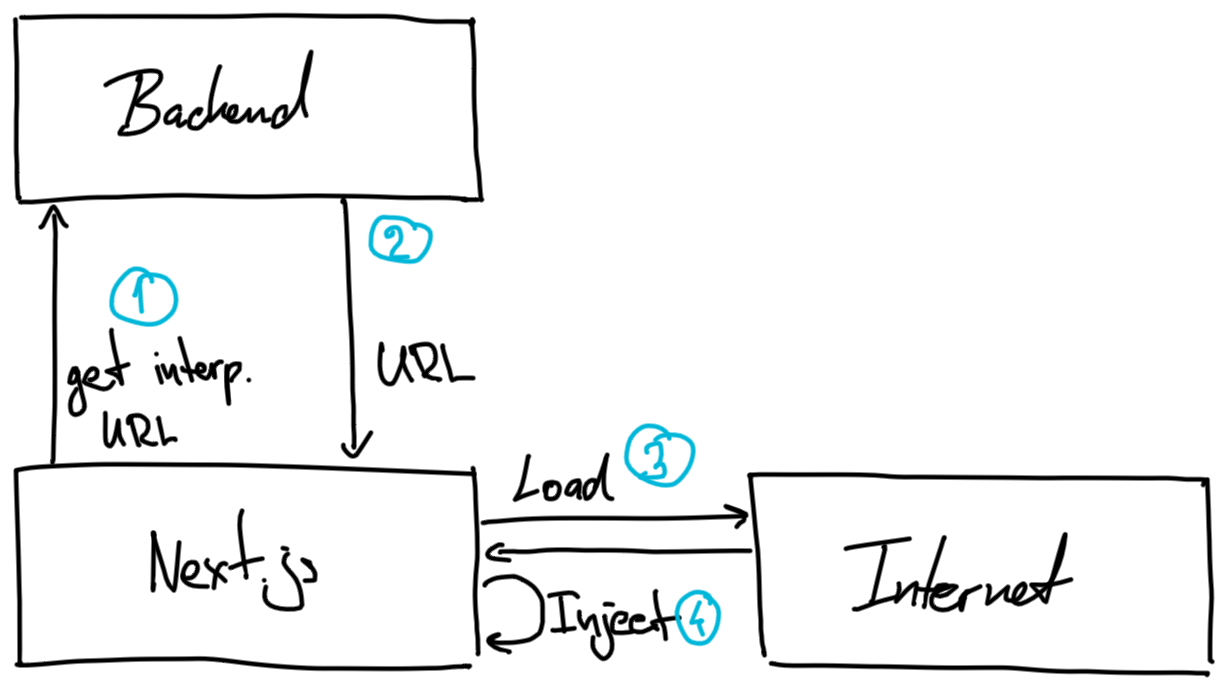
\includegraphics[max width=\textwidth]{assets/draft-fe-arch}
   \caption{Architektura klientské aplikace}\label{fig:client-arch}
\end{figure}



\section{Interprety obsahu}\label{sec:client-interpret}

Interprety obsahu tvoří jednu z těch více implementačně zajímavých částí klientské aplikace.
Dá se říct, že se jistým způsobem pokouší napodobit způsob fungování mikroslužeb na straně klienta, i když věcně se spíš chová jako doplněk.
V původní práci se jednalo o \h{.js} soubory, jež se v případě potřeby, která nastávala s prvním výskytem obsahu s vazbou na interpret, stahovaly z externích zdrojů a automaticky pouštěly.
Byly tvořeny \g{IIFE} funkcí, která do globální proměnné prostředí přidávala funkci renderování obsahu pod svým názvem.
Když se objevoval další obsah s nazvbou na stejnojmenný interpret, tak se kontrolovalo, zda renderovací funkce již existuje a opakovaně se pouštěla s informacemi dodanými ze serveru.
Výsledkem se očekával textový HTML řetězec, jenž by se mohl vložit do \g{DOM}.
Vizualizaci daného způsobu fungování lze vidět na obrázku~\ref{fig:client-interpreter-old}.

\begin{figure}[htbp]
   \centering
   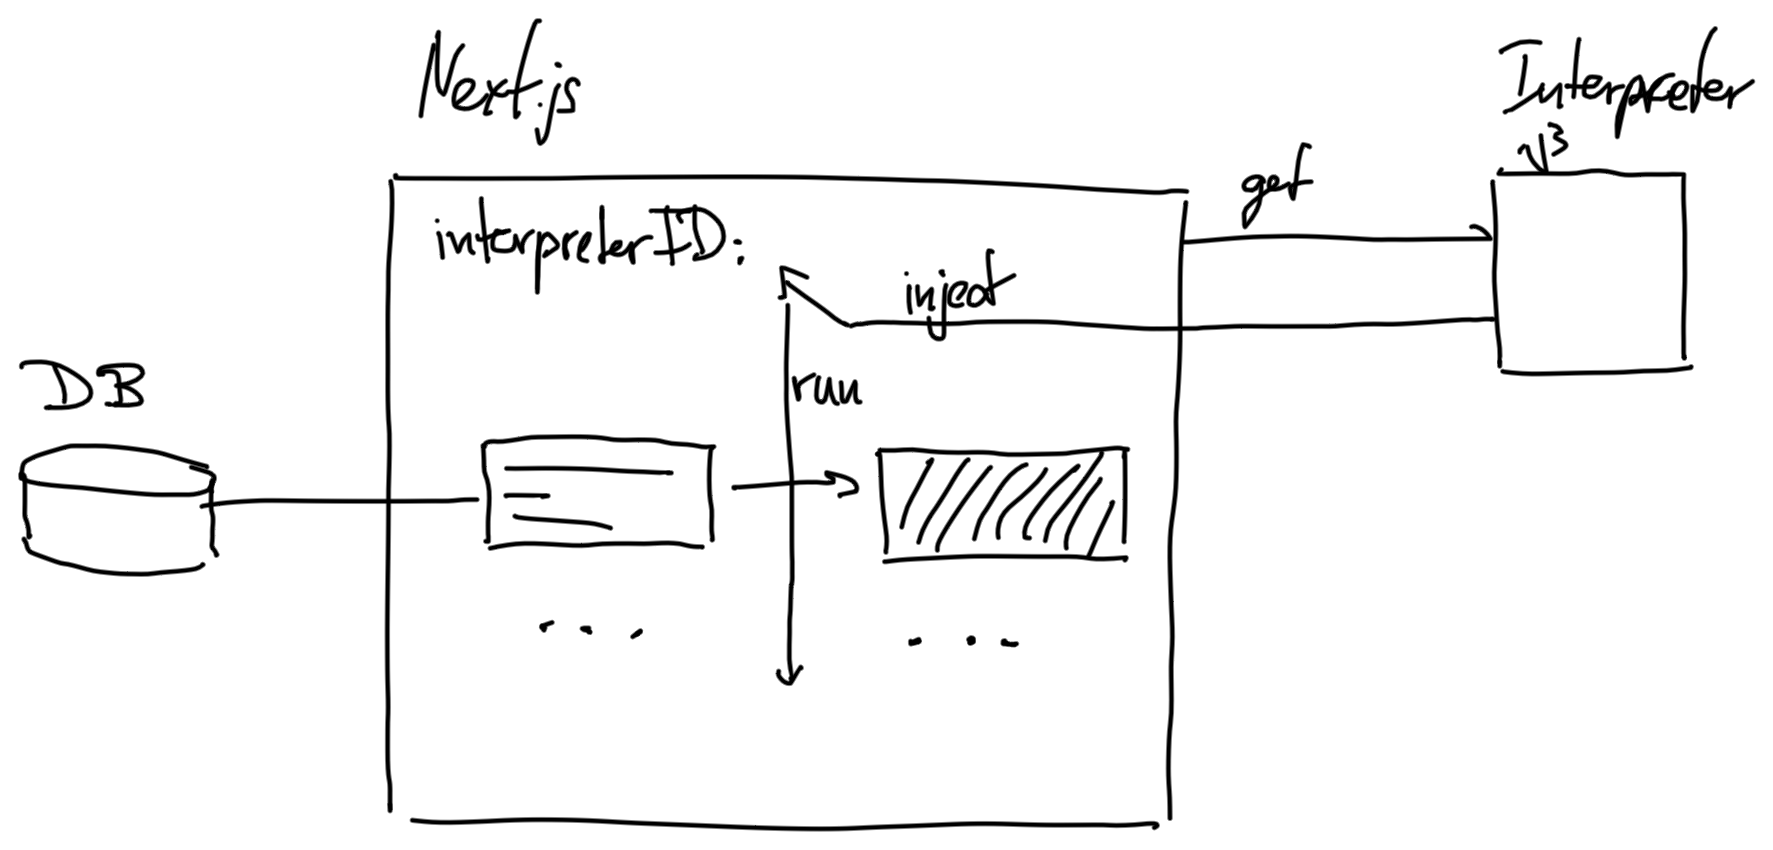
\includegraphics[max width=\textwidth]{assets/draft-interpreters}
   \caption{Původní způsob tvorby obsahů s pomocí interpretů}\label{fig:client-interpreter-old}
\end{figure}


Takový způsob nekladl žádná omezení z hlediska vybraných technologií pro interpret, ale počítal s jednoduchým vstupem (pro tvorbu jedné části obsahu se používalo jedno políčko textového obsahu) a vyžadoval validní \g{HTML} na výstupu v textové podobě.
Po vývoji několika ukázkových interpretů bylo jasné, že takový vývoj nebude zdaleka pohodlný a intuitivní.

Jako řešení se spíš nabízelo vytvořit jednoduchý interpret, který by poskytoval vestavěnou strukturu typu \h{iframe}, která by vedla na samostatný zdroj.
Tímto by se vyřešila integrace všech typů obsahů a vývoj by závisel pouze na externím dodavateli.
Po vyzkoušení implementace daného typu bylo jasné, že by se vyřešil i bezpečnostní problém vložených obsahů a separace prostředí.
Nevýhodou byla pouze nutnost existence vnějšího serveru, co by takový obsah poskytoval, což nevyhovovalo očekáváním.

Na základě takových požadavků se stanovil nový cíl který měl splnovat následující kritéria:

\begin{ul}
   \item Interpret musí být spouštěn v instanci stejné stránky, jako je samotný klient, i když se tím sníží úroveň bezpečnosti.
   \item Snížená bezpečnost může být kompenzována dotažením pouze ze známých zdrojů a zajištěním větší separace od prostředí.
   \item Interpret musí být vyvíjen v novodobých knihovnách, nejen jednoduchý \g{HTML}, aby vývojáři nemuseli obcházet nepohodlný vývoj.
   \item Tvorba dat pro interpret by měla mít formu komplexnějšího formuláře.
\end{ul}

Dané tři body ve spojení s již existující Next.js aplikací přivedly na myšlenku vestavění cizí, samostatně běžící aplikace do \g{DOM}.
Jinými slovy interpret by mohl být vyvíjen jako například samostatná React, nebo Vue aplikace a výsledek knihovny by byl rendrovaný do přesně určeného \g{DOM} elementu.

V takovém případě by se během vykreslování obsahů se Next.js aplikace starala o stažení potřebných interpretů, jako v případě původní implementace, tvorbu \h{div} elementu s unikátním \g{ID} a předávkou daného \g{ID} stažené aplikaci pro renderování poskytovaného obsahu.
Tudíž veškrá logika by se přesunula na \g{JS} kód poskytovaný interpretem.
Nevýhodou takového řešení by se však nejspíš stala velká spotřeba paměti a zpomalení aplikace jako celku, pokud by se předpokládalo, že jeden obsah projektu měl 50 částí a každá by vedla na novou puštěnou instanci knihovny.
Zároveň není jisté, jak by se choval původní React poskytovaný Next.js k obsahu, který by byl stále součástí \g{DOM}, ale pod správou jiné knihovny.

Jako řešení takové situace se nabídla redukce rozmanitosti technologií a využití toho, co již existuje – instance Next.js React, a princip, který se uplatnuje například ve Webpack – rozdělování sestavování aplikace na dynamické podmoduly, které se s pomocí běžné \g{JS} funkce pro dynamický import (\h{import('url')}) stahují v pozdějších fázích běhu aplikace.
Interpret by tudíž měl být psaný jako jednotná React komponenta s neomezeným využitím možnosti knihovny a exportovat tuto komponentu v transpilované podobě přes \g{ES6} modul.
Obdobně, druhým exportem by se mohla definovat proměnná pro popis struktury formuláře nutného pro úpravu obsahu, který by sloužil jako počáteční \h{props} do komponenty.

Během implementace se však vyskytl problém s pouštěním komponenty v existujícím React kontextu, externí komponenta po sestavení nemohla dostat přístup k Reactu jako takovému.
Proto bylo nutné odstoupit od myšlenky samostatného, běžného sestavování React aplikace a přenést vývoj do manuální podoby.
Pro vývojáře zpusob ověřování funčnosti interpretu se nezměnil – stále se jedná o komponentu v rámci samostatné React aplkace, sestavování ale vyžaduje psaní veškerého potřebného kódu v jednom souboru, manuální transpilaci například přes nástroj \h{SWC} (či jakýkoliv jiný, podmínkou je schopnost sestavování React aplikací s \h{JSX} syntaxí) a obalení výsledku funkcí, která dodává React kontext komponentě (předávání React proměnné jako argument).

Takto připravená komponenta je ve výsledku načítána do globální proměnné Next.js apliakce a vystupuje jako standardní prvek systému.
Samozřejmě takovým propojením vniklo riziko narušení funkčnosti původní aplikace, proto je důležité se k interpretům chovat jako k součástí aplikace, i když je slabě provázaná.

Takový přístup pro tvorbu interpretů byl ve výsledku zachován a byla napsána jednoduchá stavová komponenta pro vyzkoušení daného konceptu.
Dle očekávání, vznikl problém s izolací \g{CSS}, protože styly využívané s aplikaci se používaly jako výchozí pro prvky samotného obsahu.
Takovému vlivu se dá zamezit použitím například technologie \g{CSS} modulů, ale dané téma se ponechává pro další rozvoj aplikace.

Schématický vysledek fungování nové implementace interpretů je možné vidět na obrázku~\ref{fig:client-interpreter-new}.



\begin{figure}[htbp]
   \centering
   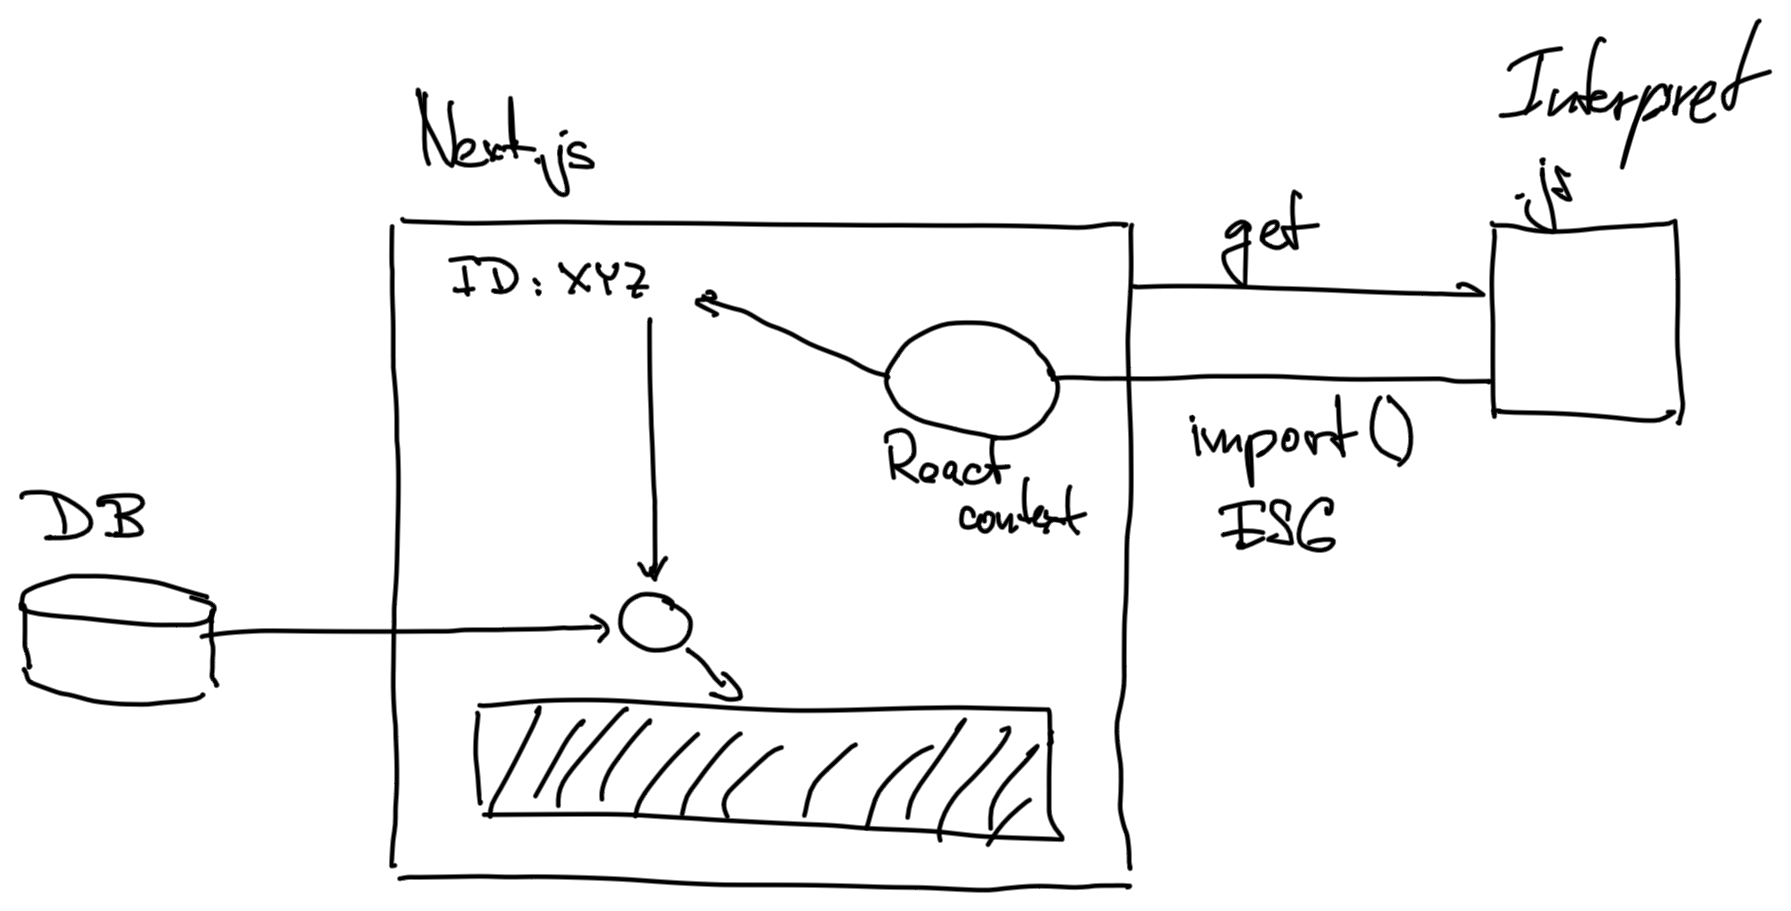
\includegraphics[max width=\textwidth]{assets/draft-interpreters-new}
   \caption{Nový způsob tvorby obsahů s pomocí interpretů}\label{fig:client-interpreter-new}
\end{figure}



\subsection{Autentizace}\label{subsec:client-auth}

Větší rozsah změn se dotknul autentizace a autorizaci uživatelů v aplikaci.
Částečně přizpůsobený OAuth 2.0 se nahradil běžnou, nezávislou implementací \enquote{access} a \enquote{refresh} tokenů pro přístup na zabezpečené zdroje.
Zjednodušil se tím postup registrace a přihlašování a eliminoval uživatelky nepříjemný manuální přechod mezi záložkami kvůli synchronizaci dat.
Za veškerou logiku získávání a obnovování tokenů nyní je zodpovědný tzv. \h{axios interceptor}.
Sekvenční diagram celého průběhu dotazování na zdroje systému s obnovou tokenů je možné vidět na obrázku~\ref{fig:cli-tokens}.


\begin{figure}[htbp]
   \centering
   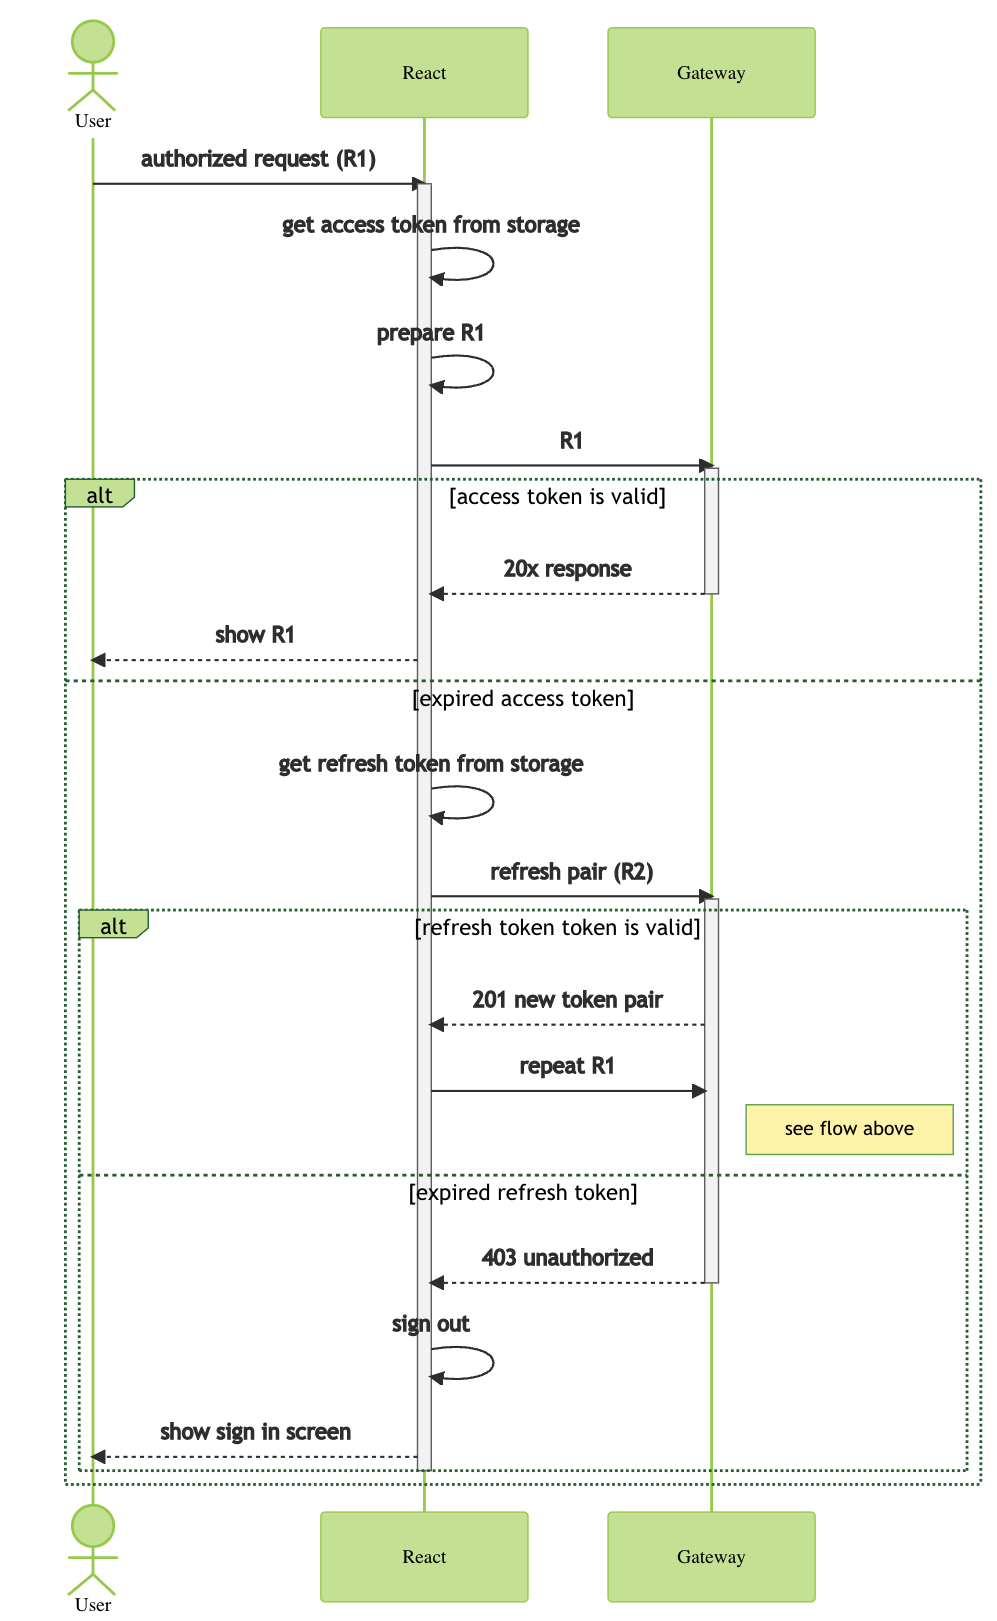
\includegraphics[max width=\textwidth]{assets/dia-seq-tokens}
   \caption{Autorizovaný požadavek a obnovení páru tokenů}\label{fig:cli-tokens}
\end{figure}



\section{Jiná zdokonalení struktury a funkcionality}\label{sec:client-improve}

Kromě dvou zásadních změn (systém interpretování obsahu a autorizace) v klientské aplikaci došlo k následujícím úpravám:

\begin{dl}
   \item[Aktualizace závislotí] – Aktualizace vyřešila problémy s instalací vyžadovaných npm balíčků a poskytla nové možnosti pro vývoj.

   \item[React hooks] – Přechod na modernější způsob zápisu React komponent s využitím \enquote{React hooks} nebyl nutný, nicméně v rámci přepisování větší části klietské aplikace bylo rozhodnuto použít nový způsob zápisu.
   Přineslo to (v porovnáním s původním kódem) výrazné snížení objemu kódu a zlepšení přehlednosti.

   \item[Nepříznivé scénáře \g{API} dotazů] – Klientské zpracování \g{API} dotazů bylo přepsáno na dotazování s pomocí obalů pro \h{Axios} knihovnu s využitím \h{React-Query}, jenž odpovídá za stav požadavků.
   To poskytuje možnost definování globálního zpracování chyb ze serveru a v příapdě speciálních situací zobrazení patřičného uživatelského oznámení.

   \item[Vizuální vzhled rozhraní] – vizuální rozhraní bylo upraveno pro lepší \g{UX}.
\end{dl}

Další změny byly menšího charakteru, rovněž však došlo k redukci z hlediska responzivního návrhu – dle nové specifikace nebyl kladen důraz na zařízení s menšími obrazovkami, aktuální řešení je přizpůsobeno pouze pro větší rozlišení, nicméně využití Bootstrap knihovny může napomoct vyřešení tohoto problému.
Daná skutečnost bylo přidána jako bod v možném budoucím rozvoji systému.
